\documentclass[a4paper,10pt]{article}
\usepackage[utf8]{inputenc}
\usepackage{graphicx}
\usepackage{url}

%opening
\title{Assignment 1: CS 763, Computer Vision}
\author{}

\begin{document}

\maketitle

\section{}
The MATLAB code is enclosed in the zip file.
We calculated the M for both datasets.
\\for dataset1:

$M$ = \[ \left( \begin{array}{cccc}
		-0.2905 & -0.0532 & 0.1866 & 0.6283\\
		0.0881 & -0.3264 & 0.0881 & 0.6010\\
		-0.0002 & -0.0002 & -0.0002 & 0.0021\\
              \end{array} \right)\] 
for dataset2:

$M$ = \[ \left( \begin{array}{cccc}
		-0.0087 & -0.0011  & 0.0039 & -0.9986\\
		-0.0001 & -0.0092 & -0.0005 &  0.0520\\
		-0.0000 & -0.0000 & -0.0000 & -0.0027\\
              \end{array} \right)\]

We added Gaussian noise by using \textbf{randn} function to each points in dataset1. After this step M was found to be

$M$ = \[ \left( \begin{array}{cccc}
    0.3024  & 0.0480 & -0.1855 & -0.6297\\
   -0.0817  & 0.3209 & -0.0929 & -0.5975\\
    0.0002  & 0.0002 &  0.0002 & -0.0021\\
              \end{array} \right)\]
              
We estimate the error by $norm(f2D - M*f3D)$. 
\\Error for dataset1: $1.2545e-10$
\\Error for dataset2: $17.2723$
\\Error with Gaussian noise in the input: $49.7882$
\\
              
Hence we can see that the eror in estimating the correct correspondence in the points lead to error in 
calibration matrix.\\
\\


\section{}

In the first part transformation in 'Hmodel.mat' is \\
\\
$Hmodel$ = \[ \left( \begin{array}{cccc}
    1.1283 &  0.0385 & -57.1714\\
    0.0702 &  1.0931 & -40.8860\\
    0.0005 &  0.0002 &  1.0000\\
              \end{array} \right)\]
and transformation got from Homography is\\
\\

$homographyTransform$ = \[ \left( \begin{array}{cccc}
    1.3241 &  0.0891 & -82.1921\\
    0.1917 &  1.2541 & -72.5790\\
    0.0003 &  0.0001 &  1.0000\\
              \end{array} \right)\]
            
            
Figure1 shows the effect of the above transformation to the images. First image is the original image,
second is the image transformed by $Hmodel$ transformation given in 'Hmodel.mat' file and third image is the image 
got from transforming the original image using transformation got from Homography(Given by $homographyTransform$).
\\
\\
\begin{figure}[ht!]
\centering
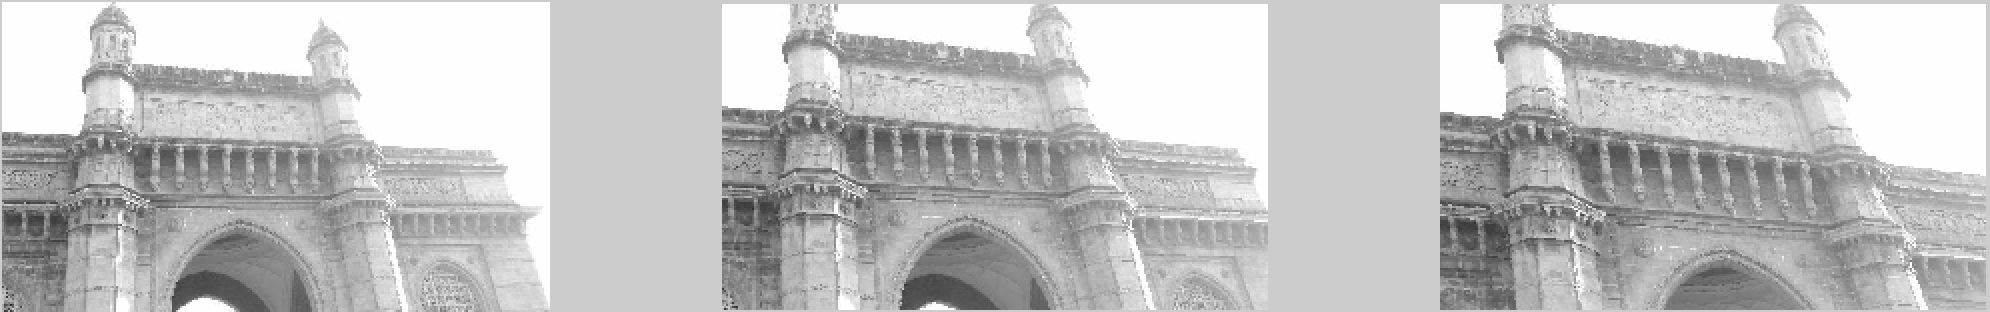
\includegraphics[width=90mm]{figure1.png}
\caption{}
\end{figure}

In the second part homography transform is \\
\\
    $homographyTransform$ = \[ \left( \begin{array}{cccc}
    0.9279 & -0.0650 & 34.1957\\
   -0.0359 &  0.8910 & 49.5626\\
   -0.0001 & -0.0002 &  1.0000\\
             \end{array} \right)\]       

Figure shows the results. First image is the original image, second is the image got from ‘goi2 downsampled.jpg’
and third is the image got from transforming the original image using the transformation got from Homography (Given by $homographyTransform$)
\begin{figure}[ht!]
\centering
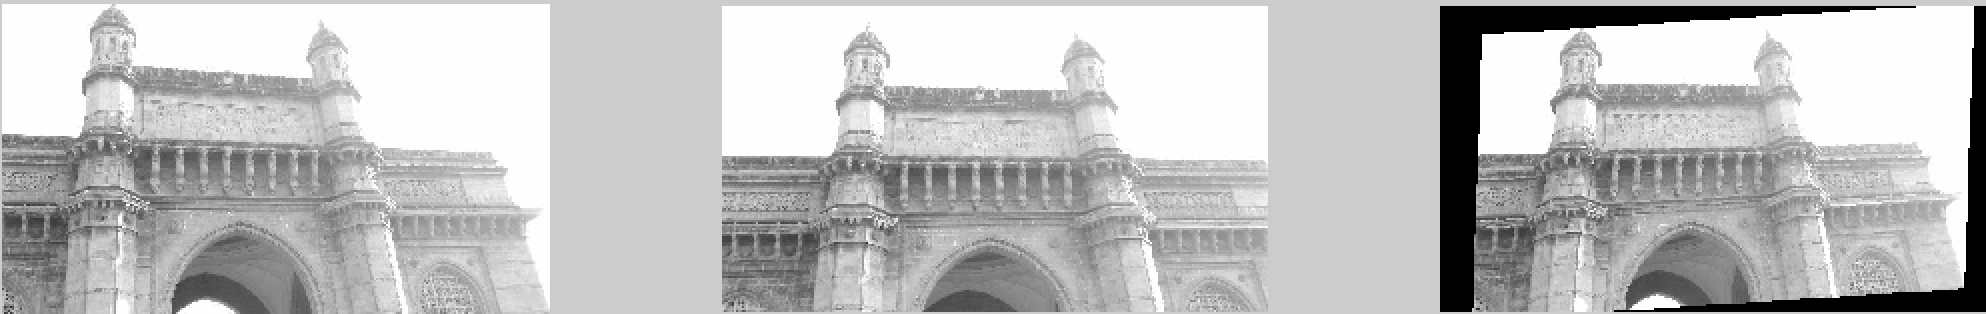
\includegraphics[width=90mm]{figure2.png}
\caption{}
\end{figure}

\end{document}
